\begin{applicationActivities}

\begin{activity}{5}
Solve the IVP \[y'=\frac{3}{2}y^\frac{1}{3}, \hspace{5em} y(1)=0.\]
\vfill
\begin{enumerate}[(A)]
\item \(y= t ^\frac{3}{2} \)
\item \(y=\left(t-1\right)^\frac{3}{2} \)
\item \(y= t ^\frac{3}{2}-1 \)
\item \(y=0\)
\end{enumerate}
\end{activity}

\begin{observation}
The ODE \(y'=\frac{3}{2}y^\frac{1}{3}\) has multiple solutions through the point \((1,0)\).

\begin{center}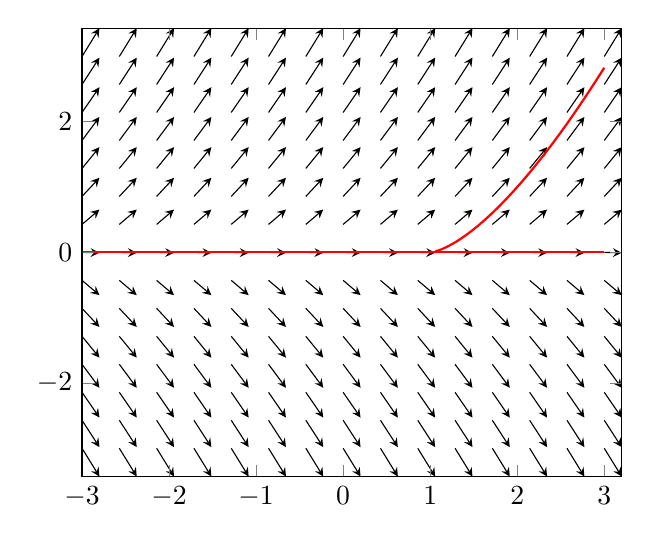
\begin{tikzpicture}
    \begin{axis}[
        domain=-3:3,
        view={0}{90},
        axis background/.style={fill=white},
    ]
        \addplot3[black,
            quiver={
             u={1},
             v={3/2*y/abs(y)*abs(y)^(1/3)},
             scale arrows=0.2,
            },
            -stealth,samples=15]
                {exp(-x) - 1/2*sin(x) - 1/2*cos(x)};
		\addplot[thick,red,domain=-3:3,samples=100]{ ((x-1))^(3/2)};
		\addplot[thick,red,domain=-3:3]{0};
    \end{axis}
\end{tikzpicture}\end{center}

\vfill
How can we guarantee our ODEs have a unique solution?

\end{observation}

\begin{observation}
Let's plot the function \(f(y)=\frac{3}{2}y^\frac{1}{3}\).\begin{center}\begin{tikzpicture}
    \begin{axis}[
        domain=-3:3,
        view={0}{90},
        axis background/.style={fill=white},
    ]
        \addplot[thick,blue,domain=-3:3,samples=100] {3/2*x/abs(x)*abs(x)^(1/3)};
    \end{axis}
\end{tikzpicture}\end{center}

\vfill
Observe: \(f(y)\) is not differentiable at \(0\)!
\end{observation}

\begin{observation}
If \(f(x,y)\) and \(\frac{\partial f}{\partial y}\) are \term{continuous} on a rectangle containing \(x_0,y_0\), then the IVP
\[ y'=f(x,y), \hspace{5em} y(x_0)=y_0\]
has a unique solution.

\vfill
The problem with our example \[y'=\frac{3}{2}y^\frac{1}{3}, \hspace{5em} y(1)=0.\]
 is that, for \(f(x,y)=\frac{3}{2} y^\frac{1}{3}\), the derivative \[\frac{\partial f}{\partial y} = \frac{1}{2} y^{-\frac{2}{3}}\] is not continuous at \((1,0)\).
\end{observation}

\begin{activity} {5}
Consider the IVP
\[ y'= \sqrt{x^2+y^2}, \hspace{5em} y(0)=0 .\]

\begin{subactivity}
Is \(f(x,y)=\sqrt{x^2+y^2}\) continuous at \((0,0)\)?
\end{subactivity}
\begin{subactivity}
Compute \(\frac{\partial f}{\partial y}\).  Is \(\frac{\partial f}{\partial y}\) continuous at \((0,0)\)?
\end{subactivity}
\begin{subactivity}
Can you conclude the IVP has a unique solution?
\end{subactivity}
\end{activity}

\begin{activity}{10}
Consider the ODE 
\[ y'= \sqrt{x^2+y^2-1}.\]

This ODE is guaranteed to have a unique solution passing through which of the following points?
\begin{enumerate}[(A)]
\item \(y(1)=1\) 
\item \(y(1)=-1\) 
\item \(y(1)=0\) 
\item \(y(0)=1\) 
\end{enumerate}
\end{activity}

\begin{activity}{10}
Consider the ODE 
\[ y'= \sqrt[3]{x^2-y^2}.\]

This ODE is guaranteed to have a unique solution passing through which of the following points?
\begin{enumerate}[(A)]
\item \(y(1)=1\) 
\item \(y(1)=-1\) 
\item \(y(1)=0\) 
\item \(y(0)=1\) 
\end{enumerate}
\end{activity}


\begin{activity}{10}
Describe all points \((x_0,y_0)\) for which the IVP
\[ y'= \ln(x^2+y^2-1) - \sqrt[3]{4-x^2-y^2}, \hspace{5em} y(x_0)=y_0\]
is guaranteed to have a unique solution.
\end{activity}


\end{applicationActivities}
